\chapter{Evaluation}
\label{chap:evaluation}

This chapter evaluates the performance of the developed fleet control system. Evaluation is done in two steps, namely in terms of assembly and motion control behavior. 

Evaluation starts with a focus on the task of automated assembly. After that, motion control performance is evaluated for two platform configurations; a single vessel scenario and a 3x1 assembled platform. Results of system behavior are presented and performance is quantified. System evaluation concludes by comparing system behavior with the design criteria discussed in section \ref{sysdesign:Architecture} 

\section{Assembly}
\label{evaluateAssembly}
This section discusses the performance of the system's ability of automated self assembly. Evaluation starts in a more general sense and ends in a quantitative manner. A variety of system responses performing assembly have been collected throughout this project from system iterations. The results that are discussed in this section are from the most final version of the platform assembly proceidure, of which the overall design is discussed in section \ref{assemblyProtocolDesign}, with minor implementational changes as discussed in section \ref{AdjustmentsAfterTests}. 

Performance of reconfiguration will be quantified by evaluating the change in relative pose between neighbouring modules in all considered degrees of freedom. Pose of vessel $j$ with respect to vessel $i$ expressed in the body fixed coordinate system of vessel $i$ is expressed as:

\begin{equation}
\eta_j^i = \begin{bmatrix} \textbf{p}^{i}_{j} \\[8pt]  \Theta_{ij} \end{bmatrix} = \begin{bmatrix} x^{i}_{j} \\[8pt]  y^{i}_{j} \\[8pt] \Psi^i_j \end{bmatrix}
\label{PerfIndicatorRelativePose}
\end{equation}


The overall system response during assembly is shown in figure \ref{AssemblyGoodGlobal_tp14}, which shows poses of the modules in the degrees of freedom of the water surface. Figure \ref{AssemblyGoodGlobal_tp14} shows that the reference heading ($\Psi$) and $x$ position remains constant during the assembly protocol. Response in $y$ direction shows pre-assembly line up at $t<295$, after which the modules approach and finally connect.  

\begin{figure}[H]
	\centering
	\captionsetup{justification=centering}
	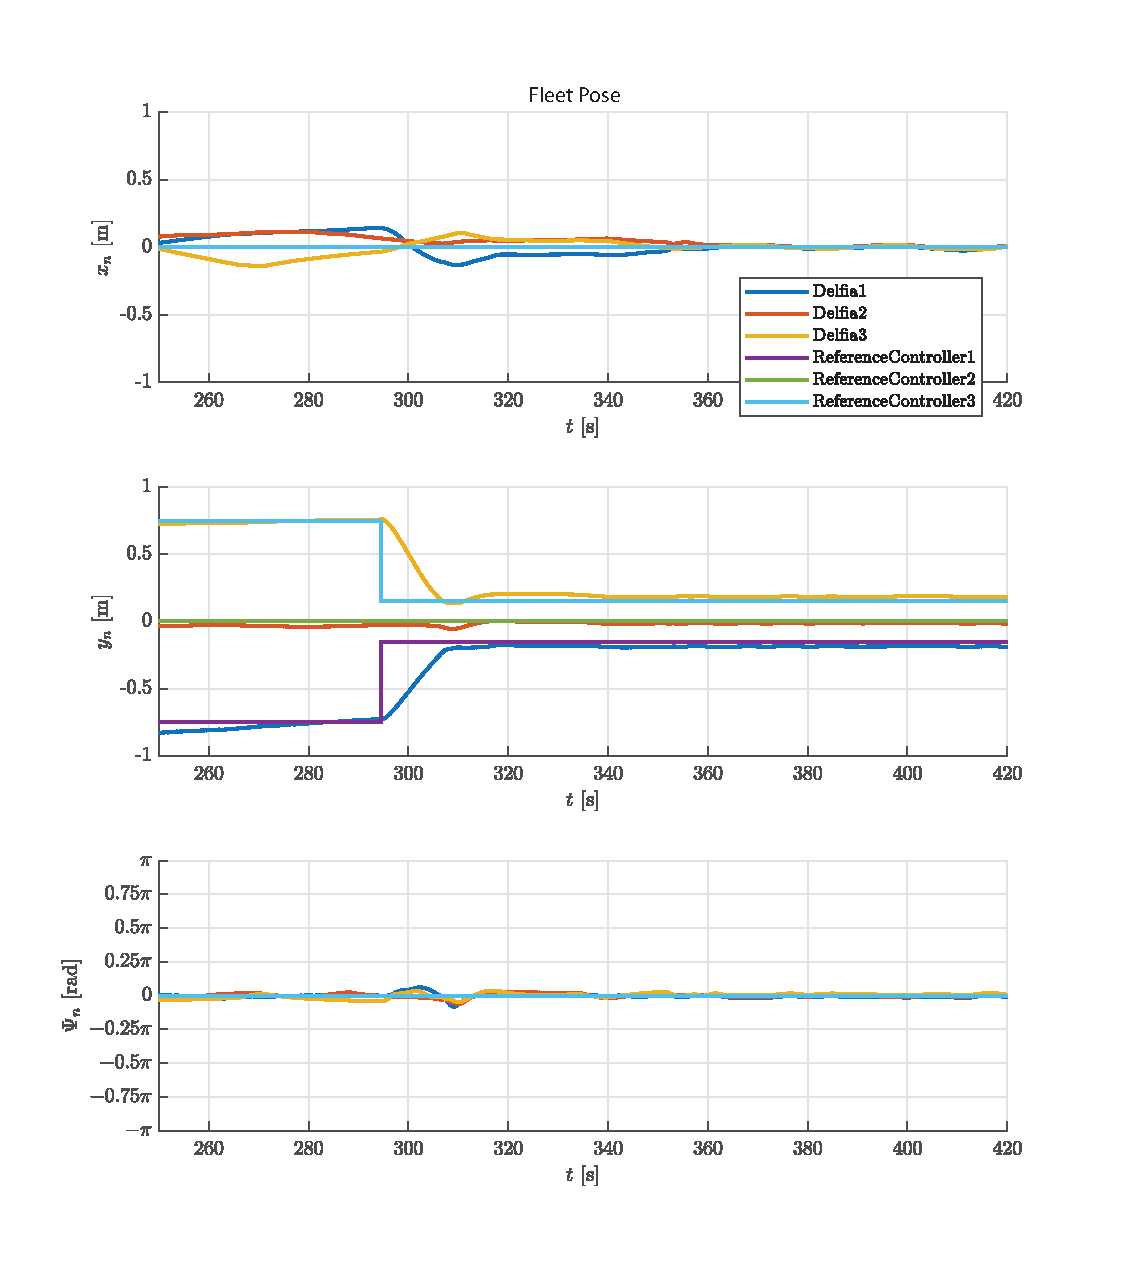
\includegraphics[width=0.9\textwidth]{VesselConnectAdjustedTotalMovementb}
	\caption{Module position plotted versus time, during the platform assembly stage. Vessels are initially lining up side-by-side, until they approach due to changin $y$ reference values. }
	\label{AssemblyGoodGlobal_tp14}
\end{figure}

Assembly succes or failure was easily detectable by eye, but can be supported quantitatively by evaluating relative motion. The two modules attempted assembly simultaneously which is shown in figure \ref{AssemblyGoodrelative_tp14}. Simultaneous plotting of relative pose of both module 1 \& 3 requires a rather large scale in $y$ direction which doesn't show a lot of detail. Therefor the relative pose of module 1 \& 3 are also individually plotted in figure \ref{connectFinal3DOF_delfia1} and \ref{connectFinal3DOF_delfia2} respectively.

\begin{figure}[H]
	\centering
	\captionsetup{justification=centering}
	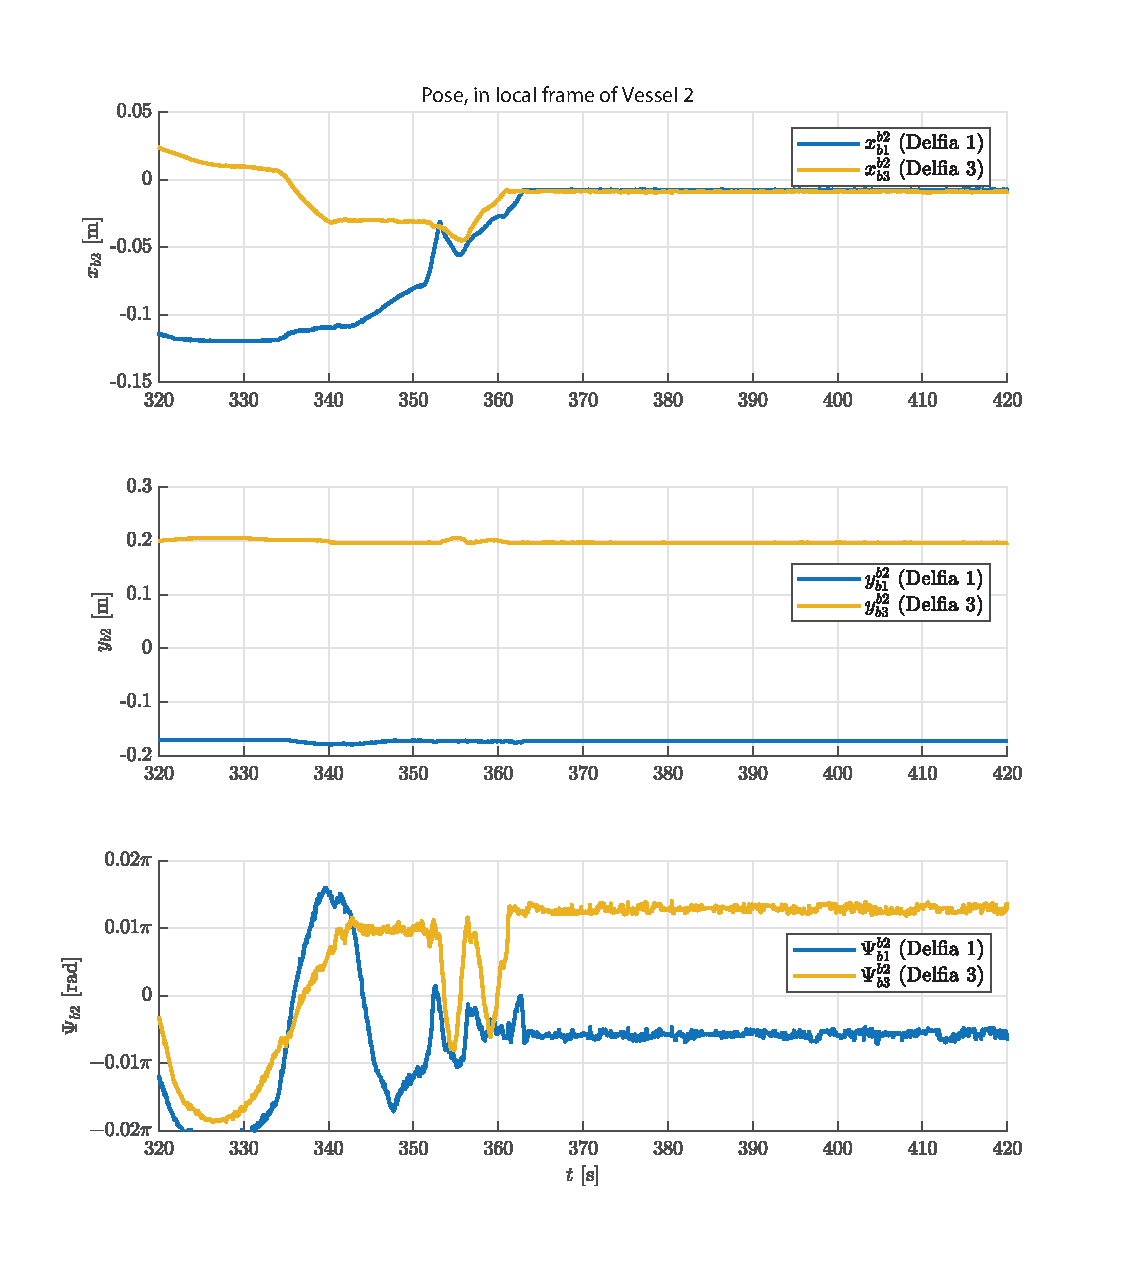
\includegraphics[width=0.9\textwidth,center]{evaluationConnect_tp14_relativemotion_wideb}%
	\caption{Relative motion of assembling vessel system}
	\label{AssemblyGoodrelative_tp14}
\end{figure} 

 \begin{figure}[H]
 	\centering
 	\captionsetup{justification=centering}
 	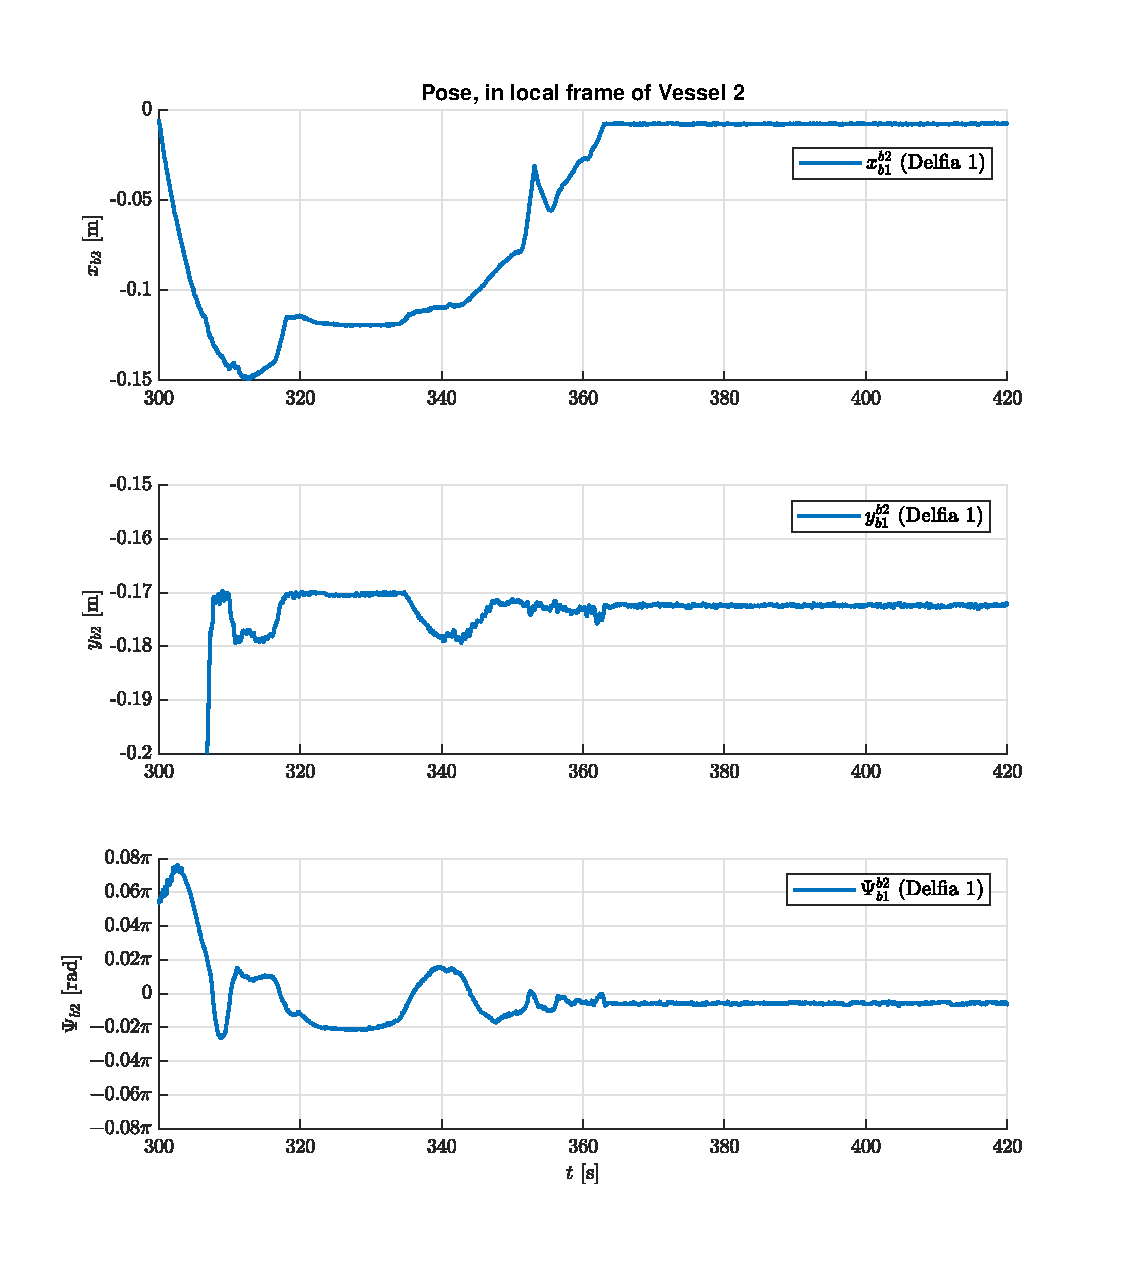
\includegraphics[width=0.9\textwidth,center]{connectFinal3DOF_delfia1}%
 	\caption{Relative motion of module 1 expressed in body fixed frame of module 2. }
 	\label{connectFinal3DOF_delfia1}
 \end{figure}

 \begin{figure}[H]
 	\centering
 	\captionsetup{justification=centering}
	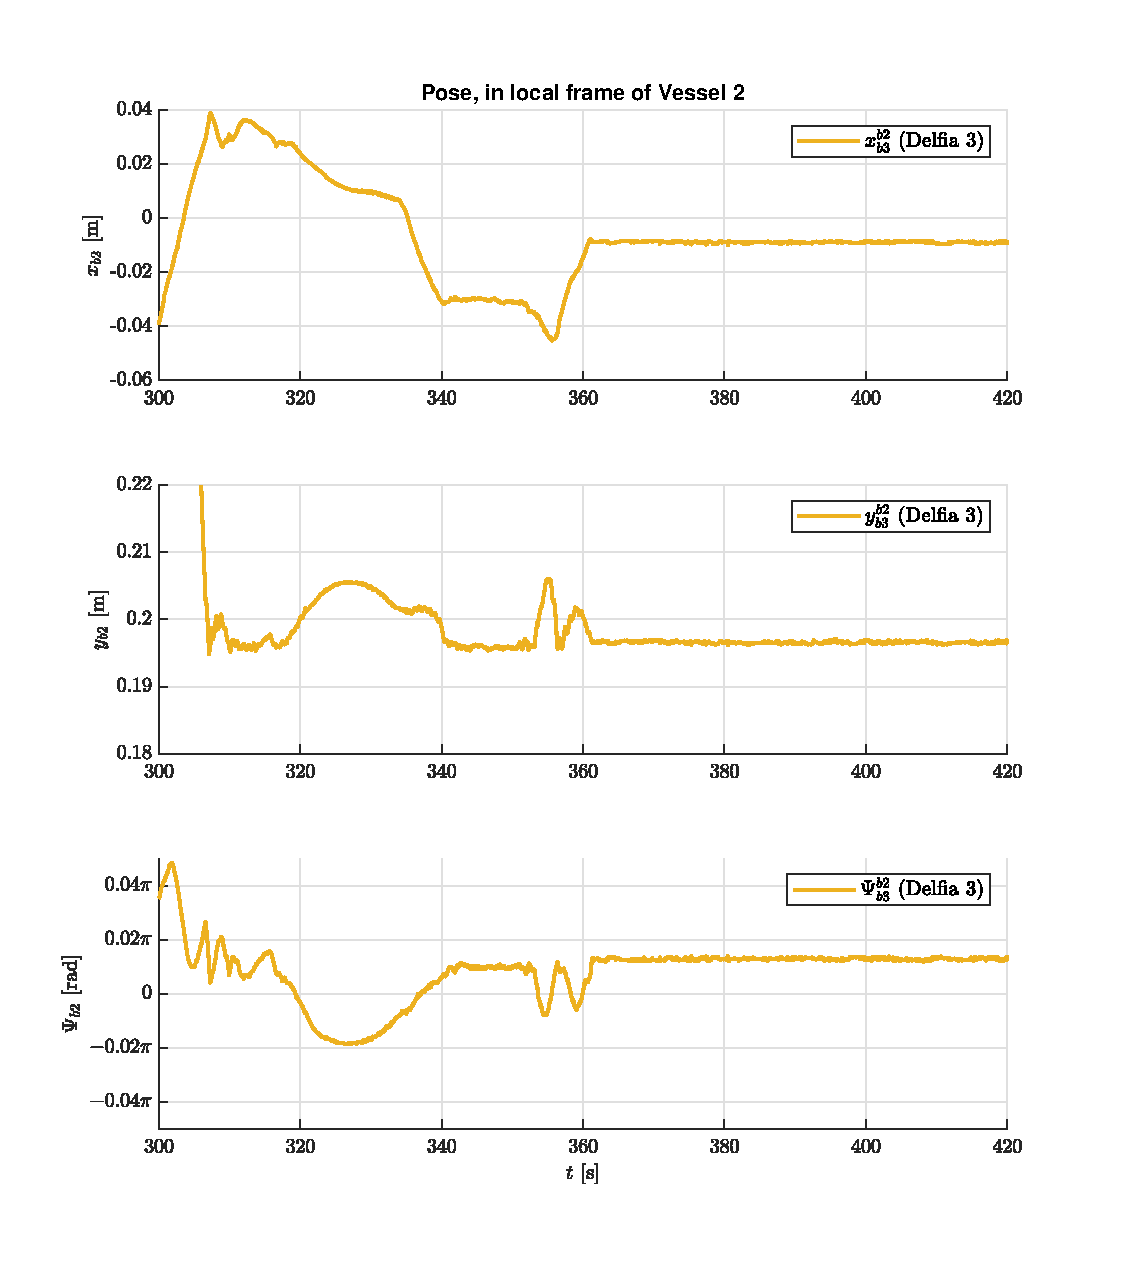
\includegraphics[width=0.9\textwidth,center]{connectFinal3DOF_delfia2}%
	\caption{Relative motion of module 3 expressed in body fixed frame of module 2.}
	\label{connectFinal3DOF_delfia2}
\end{figure}

Some notes on the module's relative positions during assembly are considered worth discussing, particularly on the interpretation of the responses. 
The signals showing relative positions in figure \ref{connectFinal3DOF_delfia1} and \ref{connectFinal3DOF_delfia2} show some forms of plateauing behavior, which is particularly interesting. The slope of these signals becoming a plateau means that relative speed has suddenly become near zero. This is considered to be due to physical contact between hulls. This can be a bump, soft contact, or a connector snapping two modules together. 
Relative pose of both connecting modules show some similarities. Pose in various DOFs show plateaus where the speed suddenly becomes near zero, which are most clear in $y$ direction for both modules. Furhermore, a clear moment can be observed on which relative motion becomes near zero for not one, but all degrees of motion, indicating a succesful connection. 

Figure \ref{fig:EvaluationConnectTwoInstances_AllDofs} to \ref{stateDuringAssembly364} illustrate how the relative motion was interpreted for module 1 at two different timestamps. At $t = 308s$ rapid descelleration, is visible in figure \ref{fig:EvaluationConnectTwoInstances_AllDofs} in $y$ direction due to hull contact, while figure \ref{stateDuringAssembly308} shows that vessel 1 is still misaligned. Some motion and aligning occurs until relative motion suddenly halts, around $t = 364s$. This shows the connector performing to restrain relative motion in configured state, shown in figure \ref{stateDuringAssembly364}.

\begin{figure}[H]
	\centering
	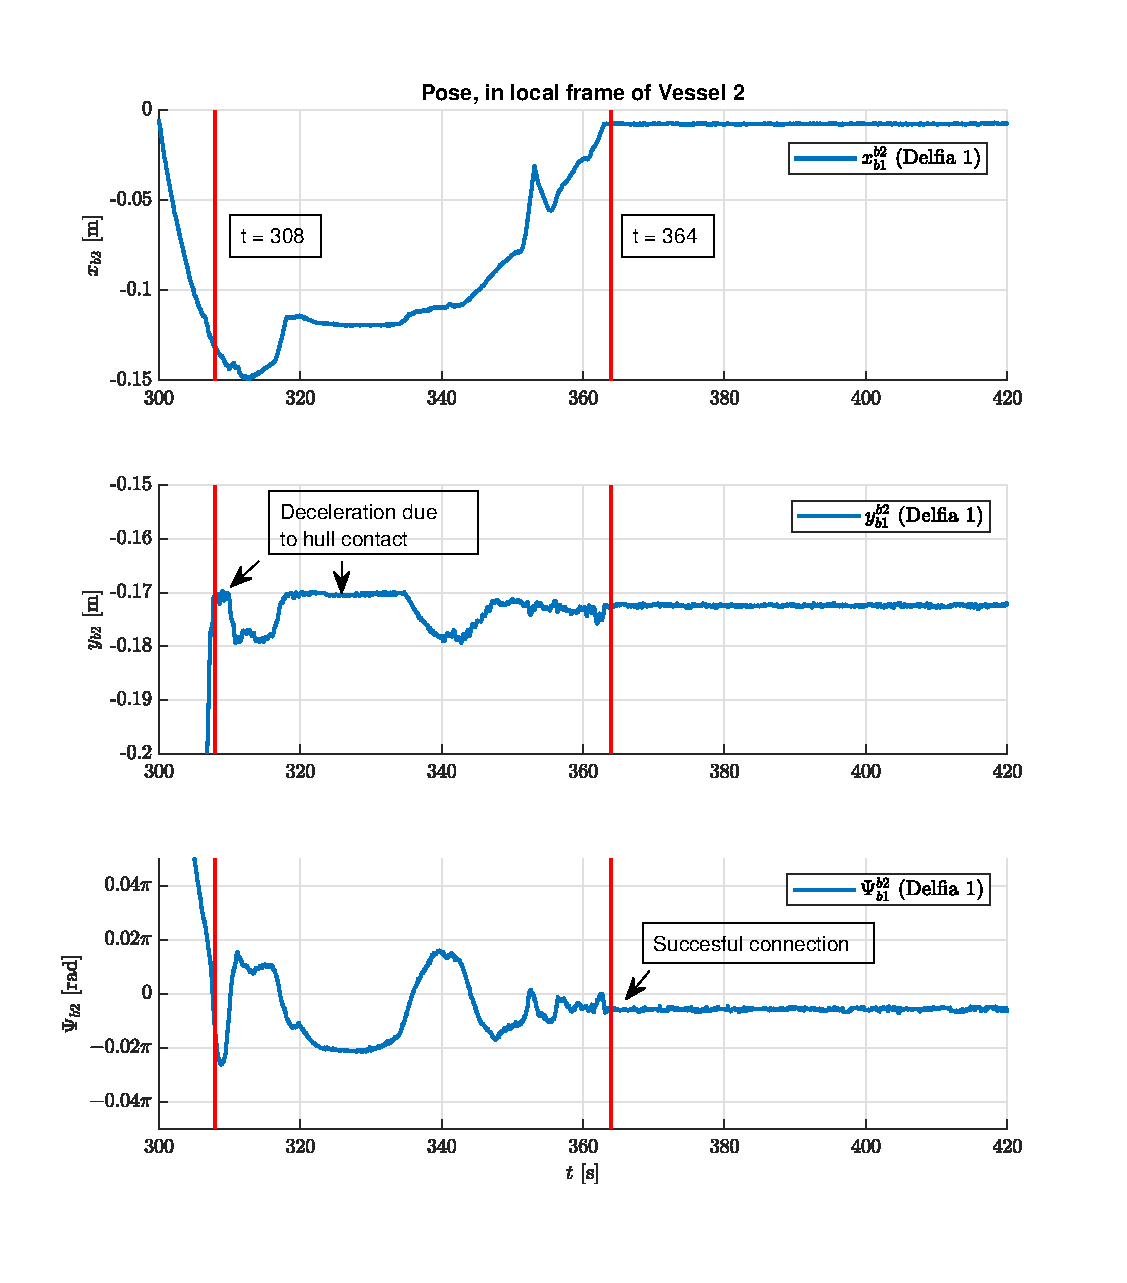
\includegraphics[width=0.9\textwidth]{EvaluationConnectTwoInstances_AllDofs2}
	\caption{EvaluationConnectTwoInstancesAllDofs}
	\label{fig:EvaluationConnectTwoInstances_AllDofs}
\end{figure}

\begin{figure}[H]
	\centering
	\makebox[\textwidth][c]{
		\begin{minipage}{0.47\textwidth}
			\centering
			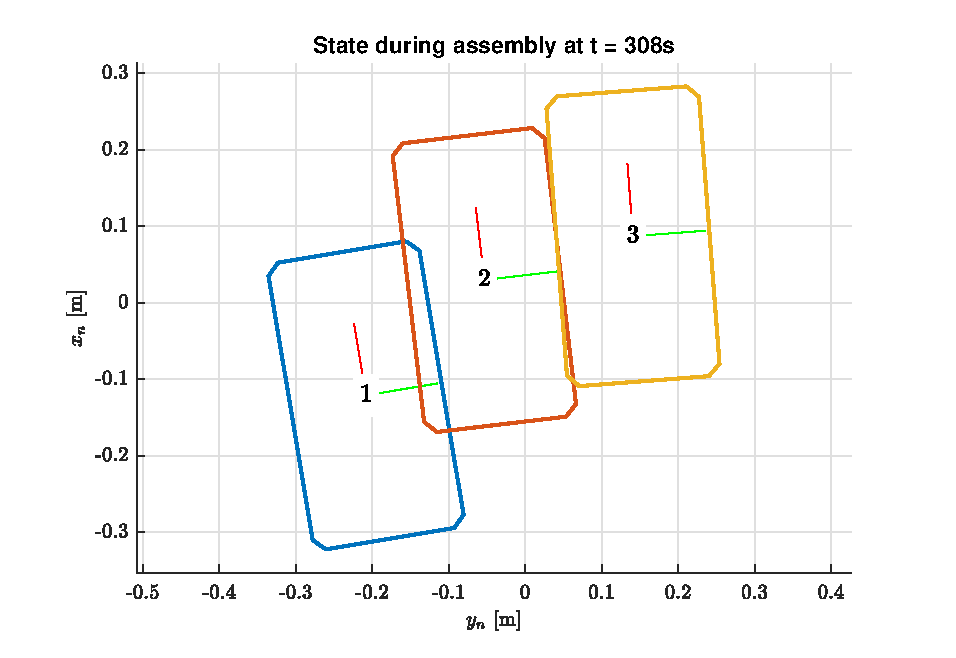
\includegraphics[width=1\textwidth]{img/stateDuringAssembly308}
			\caption{Fleet pose shown in a top-down-view at $t=308s$ while modules are aligning during assembly.}
			\label{stateDuringAssembly308}
		\end{minipage}\hfill
		\begin{minipage}{0.45\textwidth}
			\centering
			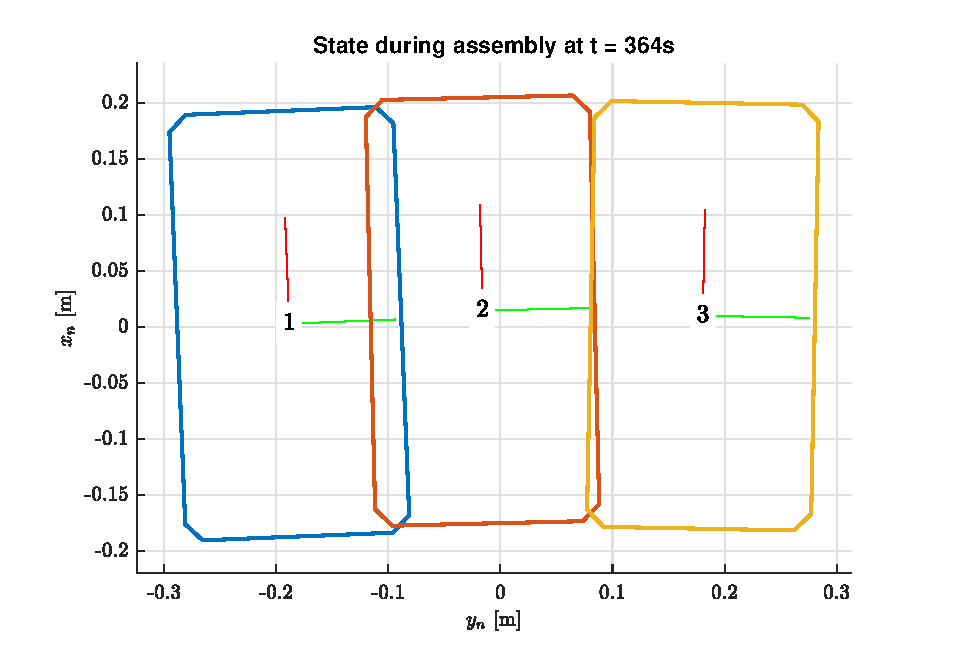
\includegraphics[width=1\textwidth]{img/stateDuringAssembly364}
			\caption{Fleet pose shown in a top-down-view at $t=364s$, as motion between modules became near zero.}
			\label{stateDuringAssembly364}
		\end{minipage}
	}
\end{figure}

To further quantify the remaining perceived motion after assembly of module 1, the dataset is evaluated from the moment of connecting (approximately at $t=364$) and 10 seconds thereafter. 

\begin{table}[H]
	\begin{tabular}{lllllll}
& & Average & Minimum & Maximum & maxAmpl & Variance \\ 
\hline 
$x$ &[m]& -0.0076628 & -0.0082233 & -0.0071825 & 0.0010408 & 4.3663e-08 \\ 
$y$ &[m]&-0.17236 & -0.17288 & -0.17198 & 0.00089951 & 2.6465e-08 \\ 
$\Psi$&[rad]& -0.018446 & -0.02136 & -0.014622 & 0.006738 & 1.0167e-06 \\ 
\hline 
\end{tabular}
	\caption{Signal analysis of relative motion of module 1 with respect to body-fixed frame of module 2 for $364<t<374$.}
	\label{tab:ConnectVariationTableOut}
\end{table}


\section{Platform Motion Control}
\label{evaluationMotionControl}
To evaluate the motion control performance of the developed framework, vessel system will be tasked to follow a time varying reference signal with step changes. Performance quantification is done by expressing rise-time and settling-time and overshoot (see fig \ref{fig:matlabStepresponseFig})of step responses to reference position of the platform in all considered degrees of freedom. Thoughout experiments steps in the platform's reference pose are given in one degree of freedom at a time. 

\begin{figure}[H]
	\centering
	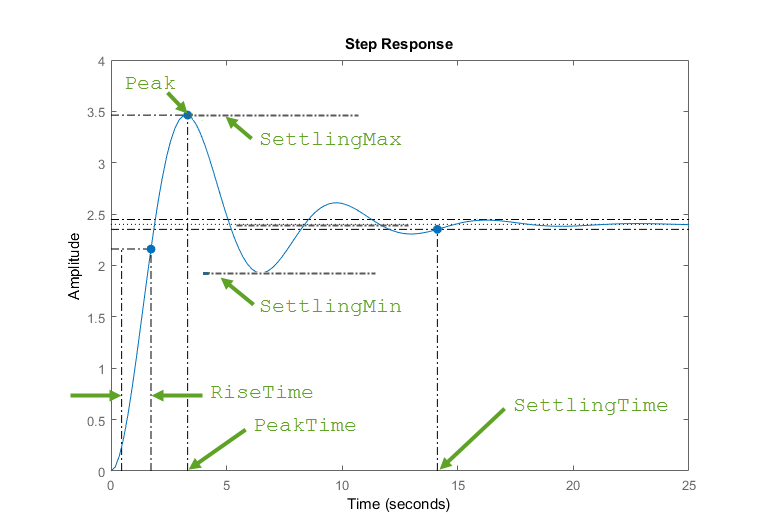
\includegraphics[width=0.7\textwidth]{stepplot1}
	\caption{Interpretation of typical quantities illustrated that are used to characterize a second order system \cite{stepinfoWebMatlab}.}
	\label{fig:matlabStepresponseFig}
\end{figure}

Platform motion is evaluated for two scenario's; single vessel operation and 3x1 lattice platform configuration, as shown in figure \ref{1x1Config} and \ref{3x1Configuration}. Note that control parameter tuning occured in single vessel operation. Any other arbitrary configuration, including the tested 3x1 platform, is required to behave satisfactory due to the configuration-adaptability of the control system. 

 \begin{figure}[H]
	\centering
	\makebox[\textwidth][c]{
		\begin{minipage}{0.47\textwidth}
			\centering
			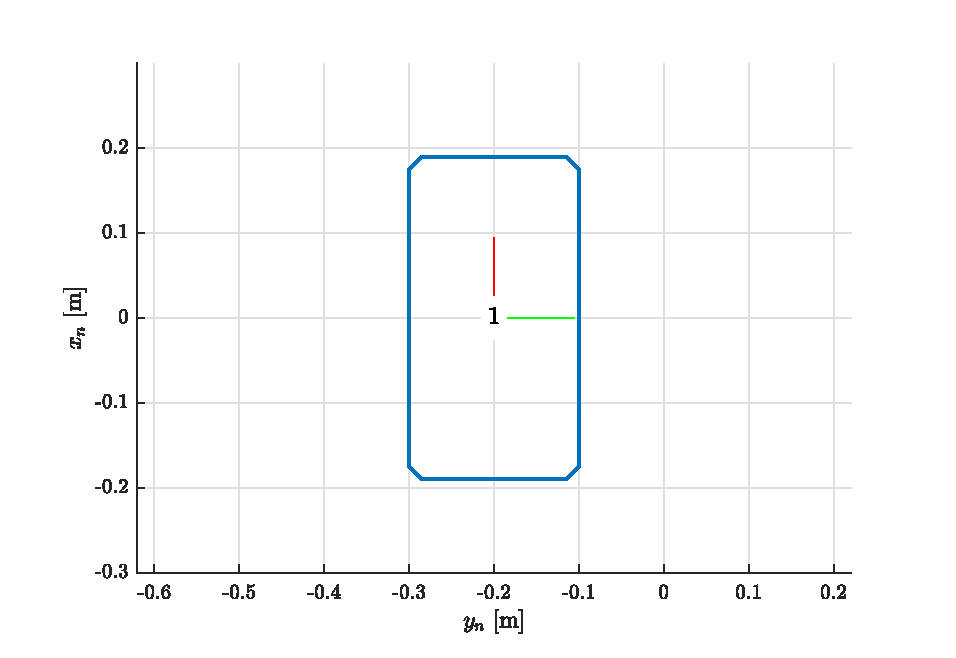
\includegraphics[width=1\textwidth]{img/1x1Config}
			\caption{A single Delfia configuration}
			\label{1x1Config}
		\end{minipage}\hfill
		\begin{minipage}{0.45\textwidth}
			\centering
			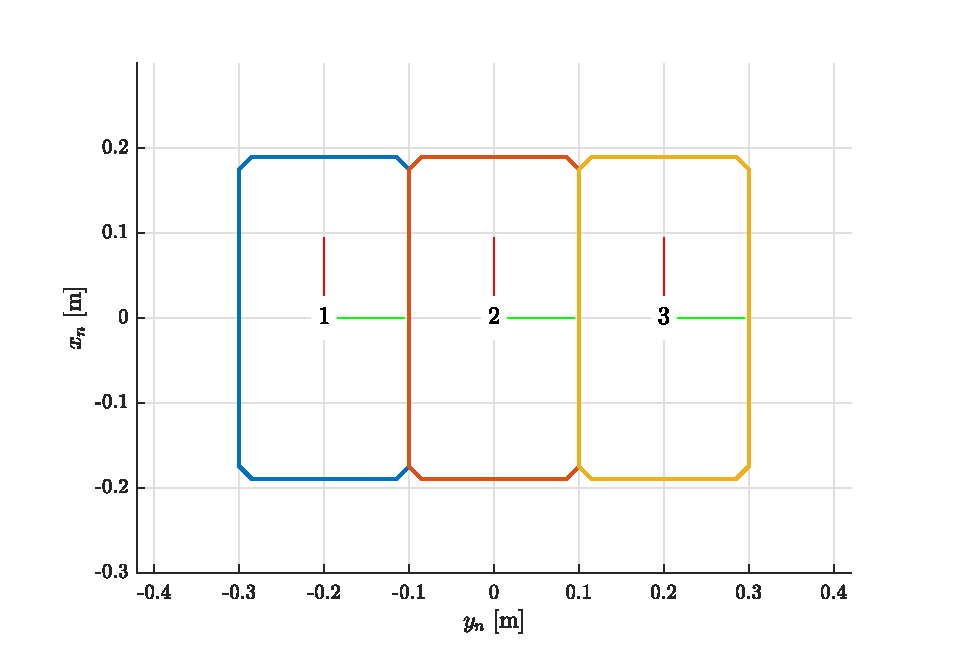
\includegraphics[width=1\textwidth]{img/3x1ConfigurationRef}
			\caption{A 3x1 platform configuration, which represented assembled platform state troughout experiments.}
			\label{3x1Configuration}
		\end{minipage}
	}
\end{figure}

Both scenarios get similar tasks of short displacements as a step input on the reference pose. These step responses are then evaluated to quantify this performance in post processing. Figure \ref{fig:tp21_steps} shows three step responses for single vessel controlled by the system. Figure \ref{fig:tp22_Steps3x} shows responses of a 3x1 configured platform. Responses of both configurations that are plotted have quantitative analysis parameters shown in tables \ref{tablev1x1} to \ref{tablev1yaw2}.

\begin{figure}[H]
	\centering
	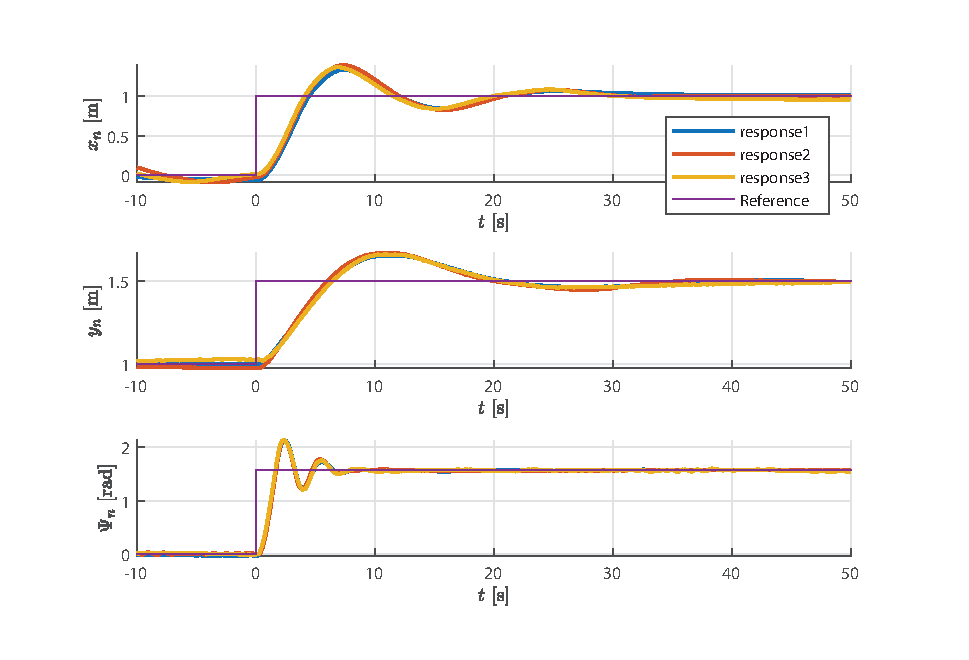
\includegraphics[width=0.8\textwidth]{tp21_stepsb.eps}
	\caption{Step responses of single Delfia configuration. Responses are gathered by changing reference of a single degree of motion (x y and yaw) at a time. Three datasets are shown, which show that the responses are rather constant.}
	\label{fig:tp21_steps}
\end{figure}

\begin{figure}[H]
	\centering
	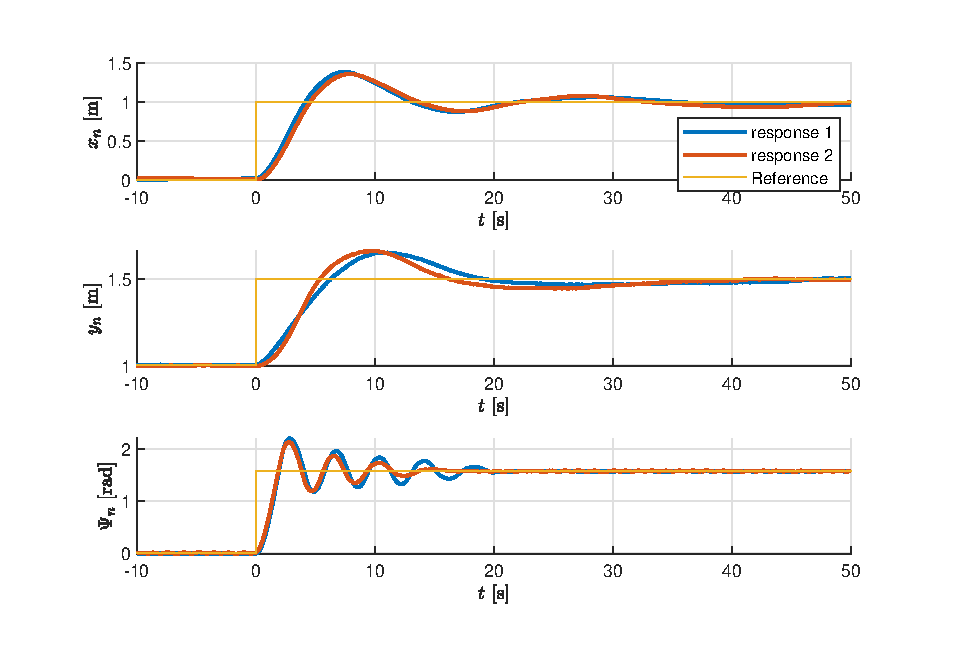
\includegraphics[width=0.8\textwidth]{tp22_Steps3xb}
	\caption{Step responses of a 3x1 lattice configuration. Responses are gathered by changing reference of a single degree of motion (x y and yaw) at a time. Two step responses are shown for each degree of motion.}
	\label{fig:tp22_Steps3x}
\end{figure}


Step responses are evaluated quantitatively in terms of rise-time, overshoot and settling-time, calculated by Matlab's 'stepinfo' function \cite{stepinfoWebMatlab}.  Rise time is defined as the time between a 10\% and 90\% rise of the signal. 
which are shown for all degrees of motion of both single and assembled configuration in tables \ref{tablev1x1} to \ref{tablev1yaw2}. The configured settling-time criteria is met if the signal is dampened within a factor of $0.05$ of the steady state value. 

\begin{table}[H]
	\captionsetup{justification=centering}
	\begin{adjustbox}{max width=1.3\textwidth,center}
		\begin{minipage}{.55\textwidth}
			\centering
			\begin{tabular}{llll}
  & RiseTime & SettlingTime & Overshoot  \\ 
  & $\;\;\;\;[s]$ & $\;\;\;\;[s]$ & $\;\;\;\;[\%]$  \\ 
\hline 
response1 & 2.803 & 27.7096 & 33.1361 \\ 
response2 & 2.3159 & 27.0722 & 38.8513  \\ 
response3 & 2.6438 & 26.6143 & 36.229  \\ 
Average & 2.5876 & 27.132 & 36.0721  \\ 
\hline 
\end{tabular}
			\caption{Single vessel $x$-direction step response evaluation}
			\label{tablev1x1}
		\end{minipage}%
		\begin{minipage}{.55\textwidth}
			\centering
			\begin{tabular}{llll}
  & RiseTime & SettlingTime & Overshoot  \\ 
  & $\;\;\;\;[s]$ & $\;\;\;\;[s]$ & $\;\;\;\;[\%]$  \\ 
\hline 
response1 & 2.9263 & 31.2773 & 38.7962  \\ 
response2 & 2.9202 & 45.2133 & 36.0778 \\ 
Average & 2.9232 & 38.2453 & 37.437  \\ 
\hline 
\end{tabular}
			\caption{Assembled 3x1 platform $x$-direction step response evaluation}
			\label{tablev1x2}
		\end{minipage}
	\end{adjustbox}
\end{table}

\begin{table}[H]
	\captionsetup{justification=centering}
	\begin{adjustbox}{max width=1.3\textwidth,center}
		\begin{minipage}{.55\textwidth}
			\centering
			\begin{tabular}{llll}
  & RiseTime & SettlingTime & Overshoot \\ 
  & $\;\;\;\;[s]$ & $\;\;\;\;[s]$ & $\;\;\;\;[\%]$  \\ 
\hline 
response1 & 4.4688 & 32.2703 & 30.6531  \\ 
response2 & 4.0913 & 31.7191 & 34.0618\\ 
response3 & 4.3417 & 35.8629 & 32.147  \\ 
Average & 4.3006 & 33.2841 & 32.2873 \\ 
\hline 
\end{tabular}
			\caption{Single vessel $y$-direction step response evaluation}
			\label{tablev1y1}
		\end{minipage}%
		\begin{minipage}{.55\textwidth}
			\centering
			\begin{tabular}{llll}
  & RiseTime & SettlingTime & Overshoot  \\ 
  & $\;\;\;\;[s]$ & $\;\;\;\;[s]$ & $\;\;\;\;[\%]$  \\ 
\hline 
response1 & 4.5348 & 32.9588 & 31.2256  \\ 
response2 & 3.3676 & 32.6829 & 33.3475 \\ 
Average & 3.9512 & 32.8209 & 32.2865  \\ 
\hline 
\end{tabular}
			\caption{Assembled 3x1 platform $y$-direction step response evaluation}
			\label{tablev1y2}
		\end{minipage}
	\end{adjustbox}
\end{table}

\begin{table}[H]
	\captionsetup{justification=centering}
	\begin{adjustbox}{max width=1.3\textwidth,center}
		\begin{minipage}{.55\textwidth}
			\centering
			\begin{tabular}{llll}
  & RiseTime & SettlingTime & Overshoot  \\ 
  & $\;\;\;\;[s]$ & $\;\;\;\;[s]$ & $\;\;\;\;[\%]$  \\ 
\hline 
response1 & 1.0576 & 6.1474 & 35.8941  \\ 
response2 & 0.97707 & 6.105 & 35.6279\\ 
response3 & 0.99748 & 6.0969 & 35.9651  \\ 
Average & 1.0107 & 6.1164 & 35.829 \\ 
\hline 
\end{tabular}
			\caption{Single vessel $\Psi$-direction step response evaluation}
			\label{tablev1yaw1}
		\end{minipage}%
		\begin{minipage}{.55\textwidth}
			\centering
			\begin{tabular}{llll}
  & RiseTime & SettlingTime & Overshoot  \\ 
  & $\;\;\;\;[s]$ & $\;\;\;\;[s]$ & $\;\;\;\;[\%]$  \\ 
\hline 
response1 & 1.2894 & 18.2124 & 40.2248  \\ 
response2 & 1.3382 & 12.8114 & 35.3374 \\ 
Average & 1.3138 & 15.5119 & 37.7811  \\ 
\hline 
\end{tabular}



			\caption{Assembled 3x1 platform $\Psi$-direction step response evaluation}
			\label{tablev1yaw2}
		\end{minipage}
	\end{adjustbox}
\end{table}


Tables \ref{tablev1x1} to \ref{tablev1yaw2} show quantitative indicators of performance of the system in two configurations. The graphs and tables show that the designed system is able to control various configurations. Step-response performance could be optimized more, but that is not the point. More important is learning from the scalability of this motion control system, as its novelty comes from using information about the platform's shape, size, and configuration. Thus, responses of single and assembled configuration will be compared. 

Recall from section \ref{controlEffortGenerationDesign} that configuration dependent platform motion control was designed with using an approximate time scale. This timescale took into account varying inertia and available control effort, with respect to the reference configuration (where reference configuration was implemented as a single vessel). 

Taking a look at the appoximate timescale for linear motion, it was found that the available thrust and inertia equally scaled linear to the amount of modules, since a homogeneous fleet is used. Thus maximum platform thrust scales as
\begin{equation}
	F_{platform,max} \approx n_{modules} * F_{single,max} 
\end{equation}
where $F_{platform,max}$ is maximum platform thrust when it fully utilizes all azimuth thrusters, $F_{single,max}$ is the maximum thrust of a single Delfia-1* module. Similarly, platform mass scales as
\begin{equation}
	m_{platform} \approx n_{modules} * m_{single} 
\end{equation}

Computing approximate time scale of linear platform motion using equation \ref{eq:timescaleDef} yields

\begin{equation}
C_{x,y} = \frac{F_{c} \; I_{ref}}{F_{ref} \; I_{c}} = 1
\label{eq:timescaleDef2}
\end{equation}
which is quite intuitive, as the maximum thrust to mass ratio remained constant.  Angular control effort and angular-inertia were appoximated to not scale similar. Values of estimated inertias and control effort are shown in table \ref{tab:inertiaAndControlEffortCompared}, which yield an approximate time constant for rotation of 

\begin{equation}
C_{\Psi}  = 1.2980
\label{eq:timescaleDefYaw}
\end{equation}
 


\begin{table}[h]
	\centering
	\captionsetup{justification=centering}
	\begin{tabular}{lll}
		& Inertia            & Maximum input  \\[10pt]  \hline
		\begin{tabular}[c]{@{}l@{}}Single vessel: \\ Translation\end{tabular}  & $4.1275kg$& $0.4320N$ \\[10pt] %\hline
		\begin{tabular}[c]{@{}l@{}}Single vessel:\\ Rotation\end{tabular} & $0.1410 kg* m^2$ & $0.0670N*m$  \\[10pt] %\hline
		\begin{tabular}[c]{@{}l@{}}3x1 Configuration:\\ Translation\end{tabular} & $12.3825 kg$  & $1.2960 N$  \\[10pt] %\hline
		\begin{tabular}[c]{@{}l@{}}3x1 Configuration:\\ Rotation\end{tabular}  & $0.7091 kg*m^2$ & $ 0.2596 N*m$   \\ \hline
	\end{tabular}
	\caption{Approximate scaling of reference and assembled configuration}
	\label{tab:inertiaAndControlEffortCompared}
\end{table}

Correctness of using the assumption of the used timescale can be evaluated by comparing response times of reference and assembled configuration. This will show to what extent the system maintains similar behavior over changing configurations, which will give indicators how it might behave for other configurations. 



\begin{table}[H]
	\centering
	\captionsetup{justification=centering}
	\begin{tabular}{lllll}
 & RiseTime & SettlingTime & Overshoot & PeakTime \\ 
 & $\;\;\;\;[s]$ & $\;\;\;\;[s]$ & $\;\;\;\;[\%]$ & $\;\;\;\;[s]$ \\ 
\hline 
Single module & 2.5876 & 27.132 & 36.0721 & 7.2288 \\
3x1 conf. & 2.9232 & 38.2453 & 37.437 & 7.6737 \\[10pt] \hline 
Ratio & 1.1297 & 1.4096 & 1.0378 & 1.0615 \\ 
\end{tabular}
	\caption{Comparison between step responses of reference (single vessel) and adapted (3x1) configuration of linear motion in x direction}
	\label{table_evaluationDifference_dimentionx}
\end{table}


\begin{table}[H]
	\centering
	\captionsetup{justification=centering}
	\begin{tabular}{lllll}
  & RiseTime & SettlingTime & Overshoot & PeakTime \\ 
 & $\;\;\;\;[s]$ & $\;\;\;\;[s]$ & $\;\;\;\;[\%]$ & $\;\;\;\;[s]$ \\ 
\hline 
Single vessel configuration & 4.3006 & 33.2841 & 32.2873 & 11.0471 \\ 
3x1 configuration & 3.9512 & 32.8209 & 32.2865 & 10.4886 \\[10pt] \hline
Ratio & 0.91876 & 0.98608 & 0.99998 & 0.94944 \\ 
\end{tabular}
	\caption{Comparison between step responses of reference (single vessel) and adapted (3x1) configuration of linear motion in y direction}
	\label{table_evaluationDifference_dimentiony}
\end{table}


\begin{table}[H]
	\centering
	\captionsetup{justification=centering}
	\begin{tabular}{lllll}
 Dimention: yaw & RiseTime & SettlingTime & Overshoot & PeakTime \\ 
 & $\;\;\;\;[s]$ & $\;\;\;\;[s]$ & $\;\;\;\;[\%]$ & $\;\;\;\;[s]$ \\ 
\hline 
Single vessel configuration & 1.0107 & 6.1164 & 35.829 & 2.3432 \\ 
3x1 configuration & 1.3138 & 15.5119 & 37.7811 & 2.8033 \\[10pt] \hline
Ratio & 1.2999 & 2.5361 & 1.0545 & 1.1964 \\ 
\end{tabular}
	\caption{Comparison between step responses of reference (single vessel) and adapted (3x1) configuration of rotational motion in yaw direction}
	\label{table_evaluationDifference_dimentionyaw}
\end{table}

To evaluate control system adaptation performance the ratio between performance indicators of reference and configured state is used from table \ref{table_evaluationDifference_dimentionx} to \ref{table_evaluationDifference_dimentionyaw}. 

\textbf{Overshoot} seems to remain rather constant, varying $3.78\%$,$0.002\%$ and $5.45\%$ for $ x$,$y$ and $\Psi$ motion respectively. 

The \textbf{rise-time} of linear motion somewhat behaves according to the approximate timeconstant of $1$ (equation \ref{eq:timescaleDef2}). The risetime ratios of $1.1297$ and $0.91876$ for x and y motion are quite near the approximated scaling of $1.0$. Differences can be explained by the fact that the implemented control system does not use directional dependent mass or dampening for linear motion. Platform mass was approximated as constant in all directions for adapting PID gains, as the position controllers used global coordinates. 

The rise-time of angular motion changed with a ratio of $1.299$, which is rather close to the approximated time constant of $C_{\Psi}  = 1.2980$ (\ref{eq:timescaleDefYaw}).

\textbf{Settling-time} varied significantly between some measurements, such as the in the x-response of the assembled configuration (table \ref{tablev1x2} settlingtimes of $31.2773$ and $45.2133$ s ). This is peculiar as the two responses in x direction plotted in figure \ref{fig:tp22_Steps3x} are very much alike. The steady state criteria was reached half a period later, but with the long periods of oscillation (in the range of ~20 seconds), this resulted in a significant difference in settling time. Applications that highly value the performance indicator of settling time are recommended to rethink appropriate settling criteria. 
Most other settling times seemed rather consistent throughout datasets, with the exception of rotation of the assembled platform. Two rotation responses of the assembled platform (figure \ref{fig:tp22_Steps3x}, $\Psi$ dimention ) show identical behavior on the first period, yet seem to show some difference in oscillation dampening, which are in line with the different settling times ( table \ref{tablev1yaw2}).

Collaborative distribution of control effort was aimed to perform in a coordinated fashion. Figure \ref{forceArrows_3x1_tp22_t84} to \ref{fig:3x3_forcePlatformMotionIllustrative} show various independent and combined modes of motion in 3x1 assembled configuration, illustrating how the control allocation protocol assigns tasks to actuators.

%\colorbox{yellow}{\parbox{12cm}{ Is this the best place to illustrate the control allocation protocol in action?}}\\

 \begin{figure}[H]
	\centering
	\makebox[\textwidth][c]{
		\begin{minipage}{0.47\textwidth}
			\centering
			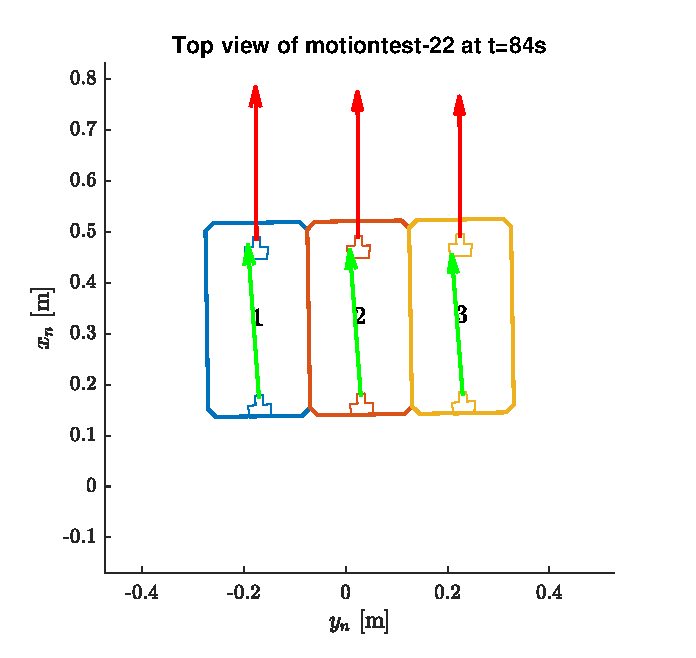
\includegraphics[width=1\textwidth]{img/forceArrows_3x1_tp22_t84}
			\caption{Control effort allocated to create (almost) pure force in x direction.}
			\label{forceArrows_3x1_tp22_t84}
		\end{minipage}\hfill
		\begin{minipage}{0.45\textwidth}
			\centering
			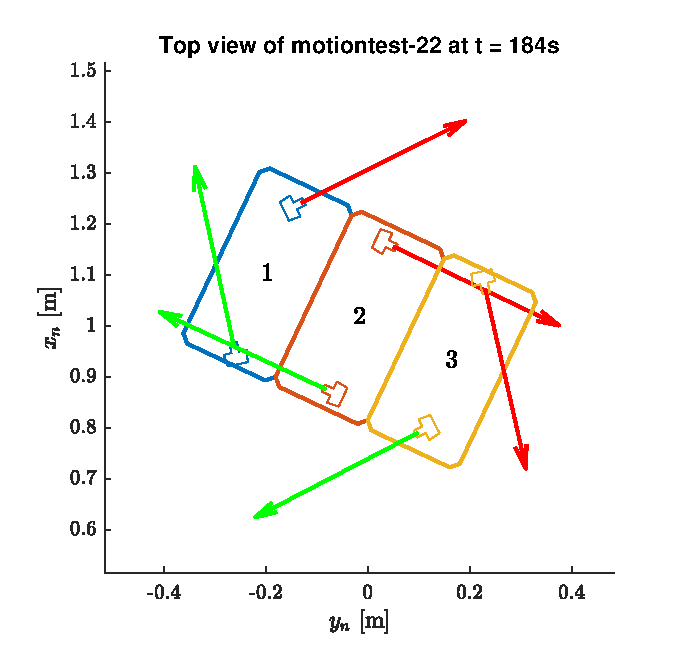
\includegraphics[width=1\textwidth]{img/forceArrows_3x1_tp22_t184}
			\caption{Control effort allocated to create pure torque about CM.}
			\label{forceArrows_3x1_tp22_t184}
		\end{minipage}
	}
\end{figure}

 \begin{figure}[H]
	\centering
	\makebox[\textwidth][c]{
		\begin{minipage}{0.47\textwidth}
			\centering
			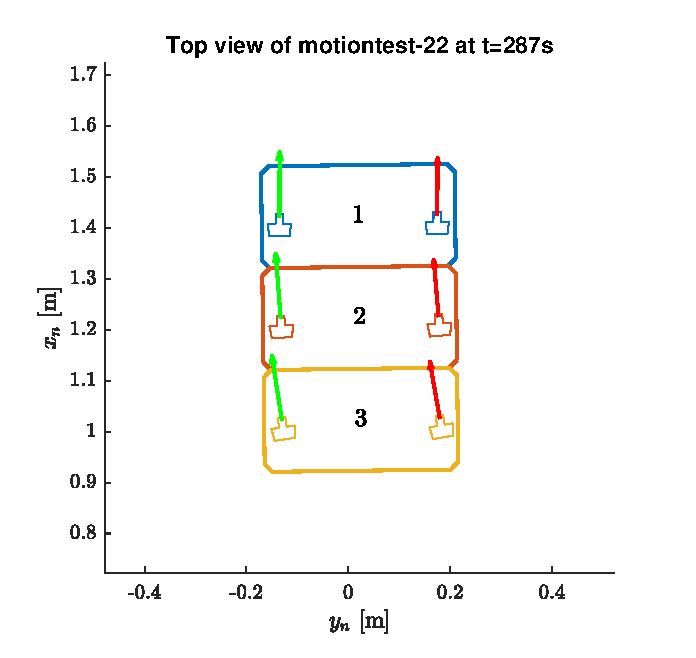
\includegraphics[width=1\textwidth]{img/forceArrows_3x1_tp22_t287}
			\caption{Control effort allocated to create (almost) pure force in body-fixed-y direction.}
			\label{X}
		\end{minipage}\hfill
	
	}
\end{figure}

\begin{figure}[H]
	\centering
	\makebox[\textwidth][c]{
		\centering
		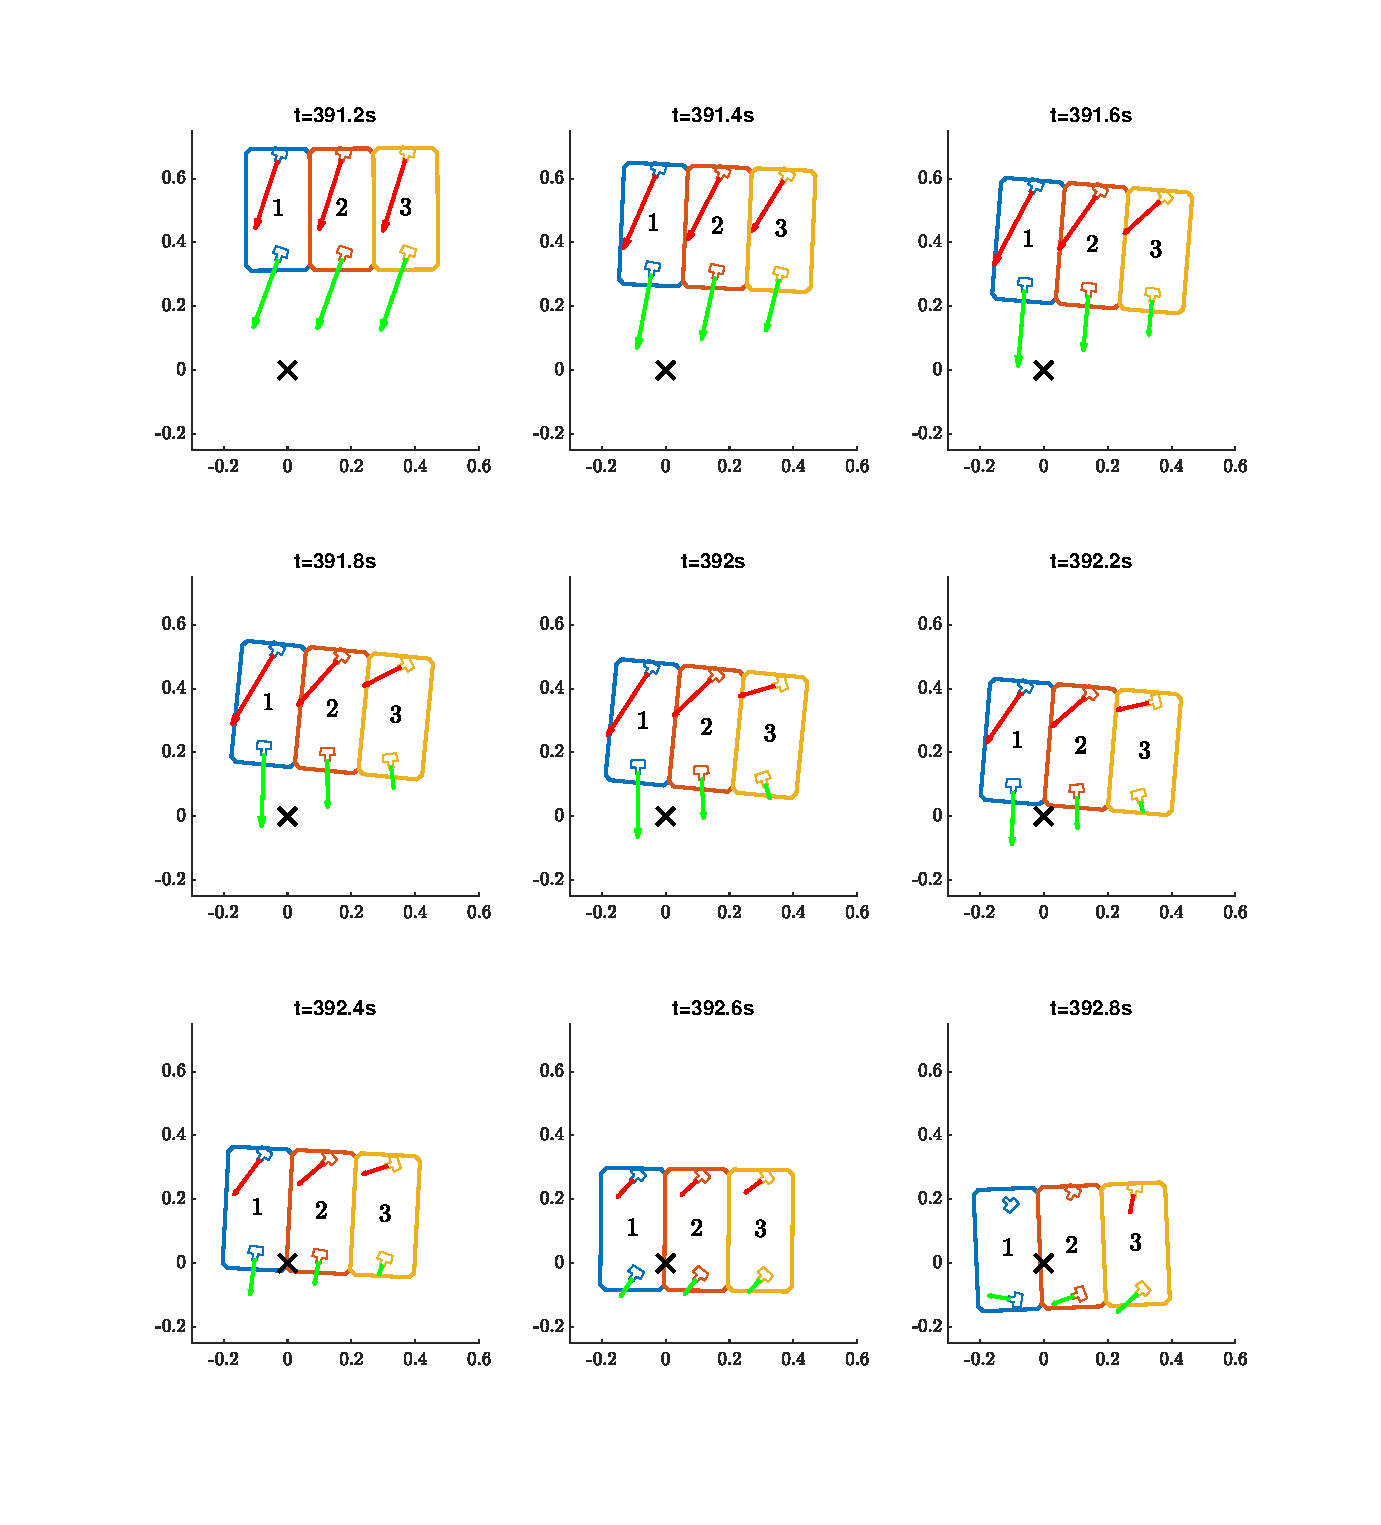
\includegraphics[width=1.3\textwidth]{3x3_forcePlatformMotionIllustrative}
	}
	\caption{Various timeframes of motiontest-22 moving to a reference position ($\times$) involving simultaneous rotation and translation. Arrows depict thruster forces, showing combined control effort (forces in various directions and torque) allocated and distributed over the platform's modules.}
	\label{fig:3x3_forcePlatformMotionIllustrative}
\end{figure}

\section{Comparing results with design criteria}

Section \ref{sysdesign:Architecture} starts describing design criteria which are evaluated here. 

Firstly, the system is required to perform automated vessel platform reconfiguration. This criteria is reached as has been observed throughout operation (by seeing magnet connectors snap into place), yet this is quantitatively supported by expressing relative module motion in section \ref{evaluateAssembly}. Figure \ref{fig:EvaluationConnectTwoInstances_AllDofs} illustrates a typical sudden stop in relative vessel motion in all degrees of freedom indicating succesful connection. Assembly of the final developed system behaved consistently throughout testing. Tab. \ref{tab:KPIresultsAssembly} shows how relative motion after connection was quantified, being near zero, compliant with the set design criteria. 

% Please add the following required packages to your document preamble:
% \usepackage{multirow}
\begin{table}[H]
	\centering
	\begin{tabular}{llllc}
		Motion & \multicolumn{1}{c}{\begin{tabular}[c]{@{}c@{}}Maximum\\ signal amplitude\end{tabular}} & Variance   & Criteria                  & \multicolumn{1}{l}{Compliant} \\ \hline
		x      & 0.0010408 m                                                                            & 4.3663e-08 & \multirow{3}{*}{$\approx 0$} & \checkmark                             \\
		y      & 0.00089951 m                                                                           & 2.6465e-08 &                           & \checkmark                             \\
		$\Psi$    & 0.006738 rad                                                                           & 1.0167e-06 &                           & \checkmark                            
	\end{tabular}
	\caption{Key performance indicators regarding assembly and compliancy versus design criteria.}
	\label{tab:KPIresultsAssembly}
\end{table}


Secondly, the system needs to perform motion control in a collaborative manner, where multiple robots work together to achieve a single goal. Centralizing platform control to a single entity facilitated modules contributing to reaching one objective and allowed coordination strategies to increase actuator usage effectiveness. Figure \ref{fig:tp22_Steps3x} displays responses to reference step changes of a 3x1 lattice configurated platform, showing how the developed system controls to converging and stabilizing at reference state. 

% Please add the following required packages to your document preamble:
% \usepackage{multirow}
\begin{table}[H]
	\centering
	\begin{tabular}{lllllll}
		\multirow{2}{*}{Configuration vs KPI} & \multicolumn{2}{c}{Risetime}                                         & \multicolumn{2}{c}{Settlingtime}                                     & \multicolumn{2}{c}{Overshoot}                                       \\
		& \multicolumn{1}{c}{Criteria}        & \multicolumn{1}{c}{Compliancy} & \multicolumn{1}{c}{Criteria}        & \multicolumn{1}{c}{Compliancy} & \multicolumn{1}{c}{Criteria}       & \multicolumn{1}{c}{Compliancy} \\ \cline{1-7} 
		Single module configuration           & \multirow{2}{*}{t\_r \textless 10s} & 100\%                          & \multirow{2}{*}{t\_s\textless{}40s} & 100\%                          & \multirow{2}{*}{os\textless{}50\%} & 100\%                          \\
		3x1 platform configuration            &                                     & 100\%                          &                                     & 83,3\%                         &                                    & 100\%                         
	\end{tabular}
	\caption{Key performance indicators regarding motion control of all degrees of motion.}
	\label{tab:KPIresultsMotion}
\end{table}


The last hard design criteria requires the developed system to perform the two abovementioned behavioral criteria simultaneously. Reconfiguration and configuration dependent platform motion control operated within the same framework, where control approach changed in troughout operation as a response to platform assembly. 

%The following evaluation is done according to criteria which were considered not crucial, yet still desirable.

The designed framework theoretically supports motion control of any arbitrary configuration, as whas desired. Experiments were conducted on two quite general shapes that both showing satisfactory responses. The control approach adapts to unknown configurations by using scaling rules aimed to be representative over a wide variety of shapes and sizes. Although scaling rules have been designed relying on physics, used assumptions need to be re-evaluated for correctness of future configurations, particularly with more extreme shapes and scales. 

The framework was developed aimed to represent a logistic solution that could be implemented in the near future. Off course full scale commercial adoption will bring some challenges that were not present in the experimental lab setup, such as disturbances due to wind and current.  All system components are considered replacable for other solutions that might better fit more realistic scales, requirements and environments. 

Replacing or improving components of the system is stimulated by making the control framework as modular as possible. Various subsystems can be further developed, which was expected as exploration of a novel combination of behaviors was the goal rather than optimization.

From this evaluation it is concluded that the system developed througout this project is compliant with the set design criteria. 


\vspace{15mm}

This evaluation and findings throughout the process of system development are presented in the next chapter to conclude this project, mention points of discussion and present the author's view on future research directions. 
